% TikZ collection file

\documentclass{article}
\usepackage[utf8]{inputenc}
\usepackage[T1]{fontenc}
\usepackage{geometry} 
\geometry{a4paper, top=25mm, left=30mm, right=20mm, bottom=30mm}
\usepackage{graphicx}
\usepackage{amsmath}
\usepackage{amssymb}
\usepackage{amsfonts}
\usepackage{tikz}
\usetikzlibrary{arrows,automata}

\title{TikZ Collection}
\author{Rene-Marcel Lehner}
\date{\today}

\begin{document}

\maketitle

\section{Basics}

% Draw an arrow with a blue dot at its base
% Draw a circle around the blue dot and a line from the blue dot to the circle. Write r on the line.
% Draw other arrows with green dots at their bases, randomly distributed around the blue dot.

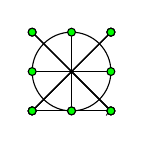
\begin{tikzpicture}
    \draw[->] (0,0) -- (1,0);
    \draw[fill=blue] (0,0) circle (0.05);
    \draw (0,0) -- (0.5,0.5);
    \draw (0.5,0.5) circle (0.5);
    \draw (0.5,0.5) -- (1,0.5);
    \draw[fill=green] (1,0.5) circle (0.05);
    \draw (0.5,0.5) -- (0.5,1);
    \draw[fill=green] (0.5,1) circle (0.05);
    \draw (0.5,0.5) -- (0,1);
    \draw[fill=green] (0,1) circle (0.05);
    \draw (0.5,0.5) -- (0,0.5);
    \draw[fill=green] (0,0.5) circle (0.05);
    \draw (0.5,0.5) -- (0.5,0);
    \draw[fill=green] (0.5,0) circle (0.05);
    \draw (0.5,0.5) -- (1,1);
    \draw[fill=green] (1,1) circle (0.05);
    \draw (0.5,0.5) -- (1,0);
    \draw[fill=green] (1,0) circle (0.05);
    \draw (0.5,0.5) -- (0,0);
    \draw[fill=green] (0,0) circle (0.05);
    \draw (0.5,0.5) -- (1,1);
    \draw[fill=green] (1,1) circle (0.05);
    \draw (0.5,0.5) -- (1,0);
    \draw[fill=green] (1,0) circle (0.05);
    \draw (0.5,0.5) -- (0,0);
    \draw[fill=green] (0,0) circle (0.05);
    \draw (0.5,0.5) -- (0,1);
    \draw[fill=green] (0,1) circle (0.05);
    \draw (0.5,0.5) -- (0.5,0);
    \draw[fill=green] (0.5,0) circle (0.05);
    \draw (0.5,0.5) -- (1,1);
    \draw[fill=green] (1,1) circle (0.05);
    \draw (0.5,0.5) -- (1,0);
    \draw[fill=green] (1,0) circle (0.05);
    \draw (0.5,0.5) -- (0,0);
    \draw[fill=green] (0,0) circle (0.05);
\end{tikzpicture}


\end{document}
